\documentclass[a4paper]{article}
\usepackage{amsmath}
\usepackage{graphicx}

\usepackage{CJK}
\begin{CJK*}{UTF8}{gbsn}

\begin{document}

%\maketitle

%
% Title Page
%
\begin{center}
	\Huge \textbf{遗传算法进行曲线拟合的办法借助观测值对电路元件参数进行估计}
\end{center}
\vspace{1 in}
\begin{center}
	\normalsize 邱铭达(1000010310) 吕一鼎(1000010679)
\end{center}
\newpage

% Contents

\tableofcontents

% Body

% 电路上的需求: 猜测电路的属性
\section{问题的产生}
在现实生活中,电路问题是一种非常重要的问题,同时它们也有着非常广泛的实际应用。其中的一类就是黑性问题,即根据某些观测值确定电路的基本构成和电学原件的值。对于直流稳恒电路来说,这是一个较为简单的问题,只要根据测量值进行一些简单的计算即可得到电路的组成情况;然而,对于含有电感、电容的非稳恒直流电路或者干脆就是交流电路来说,由于电路中存在振荡过程,一方面由于观测值存在误差,另一方面振荡过程本身不易计算,使得根据测量值来估计黑箱电路情况变得相对困难。基于这一现实情况,我们提出了这一课题——使用曲线拟合来根据少量的观测值模拟振荡电路组成状况。
%
\section{使用遗传算法进行曲线拟合}

根据问题的实际情况,我们一般知道电路的形状和具有的电子元件种类(但是不知道具体的元件
参数,这是我需要我们进行确定的),因此,可以采用遗传算法的方式,在离散化的解空间进行搜索,
通过曲线拟合的方式检验选取的元件参数是否符合我们的观测,以此达到近似确定元件参数的目的。

\subsection{遗传算法的原理}

遗传算法(Genetic Algorithm)是一类借鉴生物界的进化规律(适者生存,优胜劣汰遗传机制)
演化而来的随机化搜索方法。它是由美国的J.Holland教授1975年首先提出,其主要特点是直接对结构对象进行操作,
不存在求导和函数连续性的限定;具有内在的隐并行性和更好的全局寻优能力;采用概率化的寻优方法,能自动获取和指导优化的搜索空间
,自适应地调整搜索方向,不需要确定的规则。

遗传算法是从代表问题可能潜在的解集的一个种群(population)开始的,
而一个种群则由经过基因(gene)编码的一定数目的个体(individual)组成。
每个个体实际上是染色体(chromosome)带有特征的实体。染色体作为遗传物质的主要载体,
即多个基因的集合,其内部表现(即基因型)是某种基因组合,它决定了个体的形状的外部表现,
如黑头发的特征是由染色体中控制这一特征的某种基因组合决定的。因此,在一开始需要实现从表现型到基因型的映射即编码工作。
由于仿照基因编码的工作很复杂,我们往往进行简化,如二进制编码,初代种群产生之后,按照适者生存和优胜劣汰的原理,
逐代(generation)演化产生出越来越好的近似解,在每一代,根据问题域中个体的适应度(fitness)大小选择(selection)个体,
并借助于自然遗传学的遗传算子(genetic operators)进行组合交叉(crossover)和变异(mutation),产生出代表新的解集的种群。
这个过程将导致种群像自然进化一样的后生代种群比前代更加适应于环境,末代种群中的最优个体经过解码(decoding),可以作为问题近似最优解。

\subsection{遗传算法的实现}

针对问题我们需要对遗传算法进行具体的程序编写。考虑到遗传算法实际上并没有具体的实现方式,特别是其关键部分
(如crossover,mutation)都可以有不同的实现方法,因此重新编写代码实现一个遗传算法
代价太大。这里,我们采用 \emph{(Genetic Algorithm Utility Library)GAUL} 库提供的具体实现。

\subsubsection{Genetc Algorithm Utility Library(GAUL)}
Genetic Algorithm Utility
Library(GAUL)是一个灵活的C语言编程库,目的是为了帮助开发以遗传算法等演化算法为基础的程序。
\emph{GAUL}提供了遗传算法的核心框架,包括核心的数据类型和函数。它的灵活性表现在他可以轻松的
修改为并行执行,并设置分布式计算以加快计算速度,同时可以通过选择不同的参数使用不同的演化模型。

\subsection{程序的架构}
在程序中使用\emph{GAUL}库,核心内容是选择适当的 \emph{chromosome}
类型,实现将\emph{chromosome}翻译成问题的参数的翻译函数,并实现
对于\emph{chromosome}的\emph{fittness}的计算函数。

假设观测到的样本点是$(x_i, y_i)$,
对于指定的 \emph{chromosome} 的相应目标函数是$T(x,
\text{params})$,其中
params 是由 \emph{chromosome} 翻译过来的参数。

其中的函数$T$, 对应与程序中的函数
\begin{verbatim}
        double target_function(double x, double * params);
\end{verbatim}

对于这个问题,我们的\emph{fittness}取为负的方差
\begin{equation}
	\text{Fitness} = - \frac{\sum (y_i - T(x_i, \text{params}))}{\text{number of data points}} 
\end{equation}
对应于程序中的函数
\begin{verbatim}
        double fitting_score(population *pop, entity *entity);
\end{verbatim}

而将 chromosome 翻译为参数的翻译函数则需要针对具体问题具体确定。
这对应与程序中的函数
\begin{verbatim}
        int chromo_translator(const char * params_c, double * params_d);
\end{verbatim}

\section{具体的电路问题的解决}
由于实际的电路问题五花八门,种类丰富,所以我们仅取其中比较有代表性的两种进行分析:其一是直流情况下的RLC振荡电路,它的振荡是一个暂态过程;其二是RLC谐振电路,它是一个稳定的振荡电路,使用交流源。
\subsection{RLC-直流振荡电路}
RLC直流振荡电路是很基本的一种直流振荡电路,三极管放大器+LC振荡电路的组合是诸多家用电器的基本设计思想,比如电磁炉、电子钟等。
为使模型简化处理,我们选用了一下这张电路图:

\includegraphics[scale=0.8]{RLCzhiliu.png}

在以下分析中,E表示电源电动势,R表示串联的电阻,C表示电容,L表示电感,$U_L$表示电感的电压,$U_C$表示电容的电压,q表示电容器上的电荷,$I_L$表示流经电感的电流瞬时值,
$I_C$表示流经电容的电流瞬时值。

对于电感有自感公式:
\begin{equation}
U_L=L\frac{dI_L}{dt}
\end{equation}

对于电容有:
\begin{equation}
I_C=\frac{dq}{dt}
q=U_CC
\end{equation}

对于电阻有:
\begin{equation}
U_R=IR
\end{equation}

此时根据基尔霍夫定律有:
\begin{equation}
U_C+U_R=E
I_C+I_L=I
\end{equation}

联立得到关于$U_C$的微分方程:

\begin{equation}
\frac{d^{2}U_C}{dt^{2}}+\frac{1}{RC}\frac{dU_C}{dt}+\frac{1}{LC}U_C=0
\end{equation}
以及初值条件
\begin{align}
	&U_0 = 0 \\
	&U'_0 = \frac{E}{RC}
\end{align}

通过微分方程数值解可以得到该方程在一定$L$、一定$C$下的图像,

下面我们采用一组具体的数据进行测试。设$U = f(t)$ 是在$R=10$, $L=0.1h$, $C = 0.1F$的情况下微分方程的解,
我们假设实际测量存在着一定误差,具体的测试数据选取
(注意,虽然这里有三个参数,但实际上方程的解是由$RC,LC$ 确定的)

\begin{equation}
	U(t) = f(t) * (1 + \epsilon_t)
\end{equation}
其中$\epsilon_t$在$-0.4 \sim 0.4$之间随机取值(期望为$0$)。

通过遗传算法进行曲线拟合,可以正确的得到参数$R=10$, $L = 0.1h$, $C = 0.1F$, 

如图所示,使用基因算法拟合出的曲线与实际曲线符合得很好。

\begin{center}
\includegraphics[scale = 0.3]{rlc_fitting.png}
\end{center}

即使对于只有较少观测点的情况,通过遗传算法进行拟合也可以得到近似的结果:

\begin{center}
	\includegraphics[scale=0.3]{rlc_few.png}
\end{center}
图中的点与上述$U(t)$的取法相同。

近似拟合的结果得到$RC = 1$, $LC = 1$,
与实际结果完美的符合。

\subsection{RLC-谐振电路}

RLC谐振电路是另一类应用广泛的振荡电路,其在谐振频率振荡幅度大、偏离谐振频率震荡幅度大幅减小的特性使得此类电路大量应用于电子滤波、选频的场合,如收音机、无线电收发器等。
如下图所示,这是一张基本的串联LC谐振电路;我们的目的就是在不知道电路L、C值的情况下,通过有限的I与角频率$\omega$ 观测值,使用线性拟合的办法找出电路的谐振频率以及电感、电容的值。

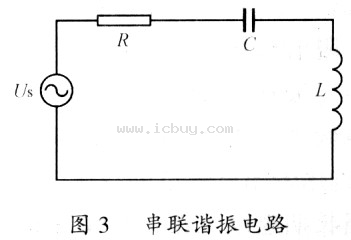
\includegraphics[scale=0.8]{RLCxiezhen.png}

由于上图为交变电路,所以选用交变电路的复数方法进行分析:

公式分析

外加交流电源$u = U\cos(\omega t + \varphi_0)$ 复数表达即$\tilde{u} = u e^{i(\omega t + \varphi_0)}$,
电阻为$R$,无相位差,即$Z_R = R$
理想情况下电感$L$, 电容$C$有抗无阻。
即$Z_L = i\omega L$, $Z_C  = \frac{1}{i\omega C} = - \frac{i}{\omega C}$ .

电路总阻抗为
\begin{equation}
	Z = Z_R + Z_L + Z_C = R + i(\omega L - \frac{1}{\omega C})
\end{equation}

相位$\theta$
\begin{align}
	& \tan \theta = \frac{\omega L - \frac{1}{\omega C}}{R} \\
	& |Z| = \sqrt{R^2 + (\omega L - \frac{1}{\omega C})^2} \\
	& Z = |Z| e^{i\theta}
\end{align}

故有
\begin{equation}
	\begin{split}
		\tilde{I} &= \frac{\tilde{U}}{\tilde{Z}} \\
				&= \frac{U}{|Z|} e^{i(\omega t + \varphi_0 - \theta)}
	\end{split}
\end{equation}

\begin{equation}
	i(\omega) = |\tilde{I}|	 = \frac{U}{\sqrt{R^2 + (\omega L - \frac{1}{\omega C})^2}}
\end{equation}

此时为了研究方便,取$\tilde{I}$的系数部分来研究其与$\omega,R,  L, C$之间的关系。

在实际生活中,以收音机为例,它的调频范围一般是$535 \sim 1600 \text{kHz}$,
所用电源一般为两节5号电池。所以在以下测试中,取电源为$3 \text{V}$交流源,调频范围$600 \sim 1600 \text{kHz}$,
先取$R = 0.1$, $C=10^{-6}$, $L=10^{-6}$来得到观测值。 
我们假设实际测量存在着一定误差,具体的测试数据选取
\begin{equation}
	I(\omega) = i(\omega) * (1 + \epsilon_\omega)
\end{equation}
其中$\epsilon_\omega$在$-0.4 \sim 0.4$之间随机取值(期望为$0$)。得到模拟的观测值以后进行测试观测值取插图

如图所示,使用基因算法拟合出的曲线与实际曲线符合得很好。

\begin{center}
\includegraphics[scale = 0.3]{iw_fitting.png}
\end{center}

即使对于只有较少观测点的情况,通过遗传算法进行拟合也可以得到近似的结果:

\begin{center}
	\includegraphics[scale=0.3]{iw_few.png}
\end{center}
图中的点与上述$U(t)$的取法相同。

近似拟合的结果得到$R = 0.8$, $L= 10^{-6}$, $C = 10^{-6}$,
与实际结果近似符合。

\section{总结}

本论文研究了一种通过遗传算法进行曲线拟合的方法,从有限的观测值出发分析
电路的元件情况的方法。在实际研究中,经常会碰到了解电路的元件组成
但不清楚具体元件的参数的情况,这是,可以通过对电路通电,随时间随电压
等参数的变化,进行观测,记录数据,对这些数据做遗传算法曲线拟合,近似
估计各个电路元件的参数。

遗传算法是基于自然研究的搜索算法,它能够很好的发现近似最优解,同时
不容易陷入局部最优“陷阱”,同时它的收敛一般比较优秀,使得遗传算法在许多领域
都有广泛的应用。

这篇文章提供了两个例子以现实遗传算法进行参数估计的有效性,它现实了
这个算法对于电子领域电路分析特定问题的研究的价值。

\section{参考文献}
[1] C.L.Karr,B.Weck,D.L.Massart,P.Vankeerberghen.Least Median Squares Curve Fitting Using a Genetic Algorithm[J].The Great Britain:EngngApplic. Artif. lntell. 1995,Vol. 8, No. 2:177-189.

[2] Fujiichi Yoshimoto,Toshinobu Harada,Yoshihide Yoshimoto.Data Fitting with a Spline Using a Real-coded Genetic Algorithm[J].The United States:Computer-Aided Design, 2003,35:751-760. 

[3] Paul Horowitz, Winfield Hill.The art of electronics[M].The Great Britain:Cambridge University Press 

[4] 赵凯华,陈熙谋.电磁学[M].北京:高等教育出版社
\end{CJK*}
\end{document}
